\documentclass[compress,red]{beamer}
\usepackage[utf8]{inputenc}
\usepackage{ucs}
\usepackage{amsmath}
\usepackage{amsfonts}
\usepackage{amssymb}
\usepackage[russian]{babel}
\usepackage{graphicx}
\usepackage{wrapfig}

\usepackage{tikz}
\usepackage{verbatim}

\usepackage{color}
\usepackage{xcolor}
\usepackage{listings}

\usepackage{caption}
\DeclareCaptionFont{white}{\color{white}}
\DeclareCaptionFormat{listing}{\colorbox{gray}{\parbox{\textwidth}{#1#2#3}}}
\captionsetup[lstlisting]{format=listing,labelfont=white,textfont=white}

\usetikzlibrary{calc,trees,positioning,arrows,chains,shapes.geometric,%
    decorations.pathreplacing,decorations.pathmorphing,shapes,%
    matrix,shapes.symbols}

\tikzset{
>=stealth',
  punktchain/.style={
    rectangle, 
    rounded corners, 
    % fill=black!10,
    draw=black, very thick,
    text width=10em, 
    minimum height=3em, 
    text centered, 
    on chain},
  line/.style={draw, thick, <-},
  element/.style={
    tape,
    top color=white,
    bottom color=blue!50!black!60!,
    minimum width=8em,
    draw=blue!40!black!90, very thick,
    text width=10em, 
    minimum height=1.5em, 
    text centered, 
    on chain},
  every join/.style={->, thick,shorten <=1pt},
  decoration={brace},
  tuborg/.style={decorate},
  tubnode/.style={midway, right=2pt},
}

\mode<presentation>

\usetheme{Warsaw}

\definecolor{Red}{rgb}{1,0,0}
\definecolor{Blue}{rgb}{0,0,1}
\definecolor{Green}{rgb}{0,1,0}
\definecolor{magenta}{rgb}{1,0,.6}
\definecolor{lightblue}{rgb}{0,.5,1}
\definecolor{lightpurple}{rgb}{.6,.4,1}
\definecolor{gold}{rgb}{.6,.5,0}
\definecolor{orange}{rgb}{1,0.4,0}
\definecolor{hotpink}{rgb}{1,0,0.5}
\definecolor{newcolor2}{rgb}{.5,.3,.5}
\definecolor{newcolor}{rgb}{0,.3,1}
\definecolor{newcolor3}{rgb}{1,0,.35}
\definecolor{darkgreen1}{rgb}{0, .35, 0}
\definecolor{darkgreen}{rgb}{0, .6, 0}
\definecolor{darkred}{rgb}{.75,0,0}

\xdefinecolor{olive}{cmyk}{0.64,0,0.95,0.4}
\xdefinecolor{purpleish}{cmyk}{0.75,0.75,0,0}

\useoutertheme[subsection=false]{smoothbars}

\title{Сервисы Google}
\author{Информационные технологии}

%\usecolortheme{dolphin}


\begin{document}
%%титульная страница
\maketitle
%% основные моменты

\section{Веб 2.0}
\subsection{Эпоха веб 2.0}
\begin{frame}
\frametitle{Эпоха веб 2.0}
		\begin{itemize}
		\item Первые сайты в Интернете выполняли функции хранения информации.
		\item Передача информации осуществлялась в одну сторону --- от владельца сайта к пользователю.
		\item Постепенно стала появляться динамика --- от гостевых книг и форумов до первых сервисов по созданию сайтов, блогов и др.
		\item Случившийся в конце 90-х --- начале 2000-х годов \emph{кризис доткомов} существенно ``почистил'' список компаний.
		\item В 2004--2005 годах Тимом О'Рейли (основатель O'Reilly Media) было выдвинуто определение ``нового веба'': 
		\end{itemize}
		\begin{quote}
		   Веб 2.0 --- методика проектирования систем, которые путём учета сетевых взаимодействий становятся тем лучше, чем больше людей ими пользуются.
		\end{quote}
\end{frame}

\subsection{Особенности веб 2.0}
\begin{frame}
\frametitle{Особенности веб 2.0}
		\begin{itemize}
		\item Строго говоря, термин веб 2.0 не является научным. По поводу того, что же это такое, споры ведутся до сих пор.
		\item Можно выделить несколько ключевых аспектов идеологии веб 2.0, ставших сейчас уже для нас нормой:
		  \begin{enumerate}
		    \item Веб-служба и SaaS--модель: ПО содержится в Интернете на серверах компании, которая создала службу. Всегда самая свежая версия, не надо думать об обновлениях и поддержке.
		    \item AJAX (асинхронный javascript) --- передача информации без перезагрузки страницы.
		    \item Социализация --- от анонимности к персонализации. Создание глобальных социальных сетей и их интеграция с другими сервисами.
		    \item Мэшапы --- сервисы, использующие в качестве источников информации другие сайты и предоставляющие более удобный доступ к данным.
		  \end{enumerate}
		\end{itemize}
\end{frame}

\section{GMail и G+}
\subsection{Сервисы}
\begin{frame}
  \frametitle{GMail обычный}
	\centerline{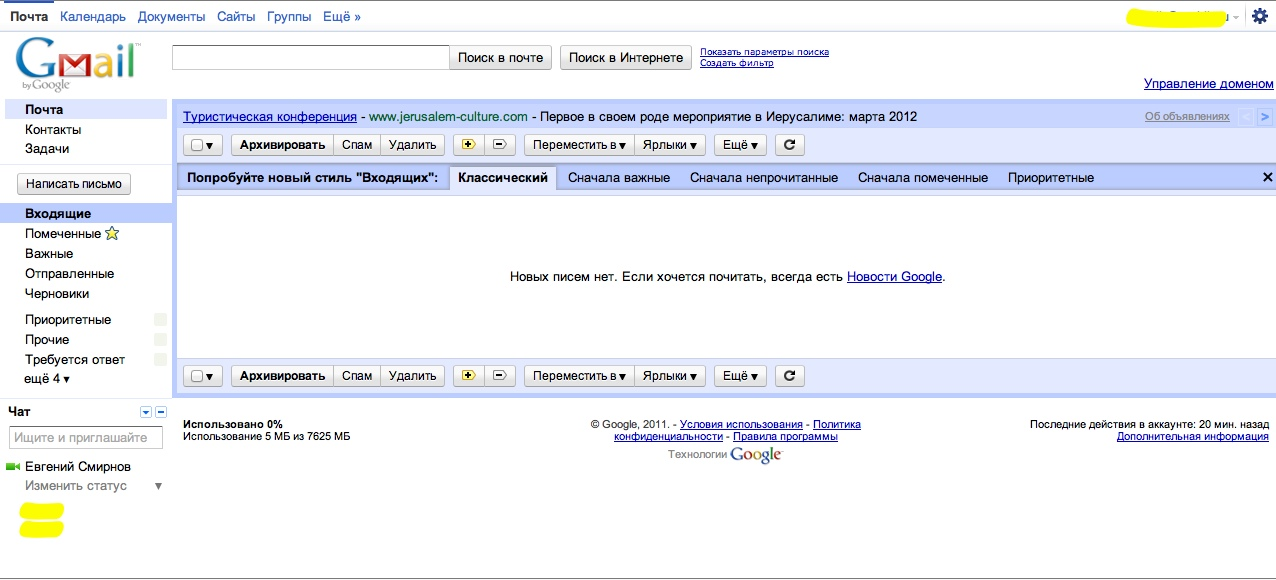
\includegraphics[width=1.0\textwidth]{images/gmail-default.jpg}}
\end{frame}

\subsection{Сервисы}
\begin{frame}
  \frametitle{GMail современный}
	\centerline{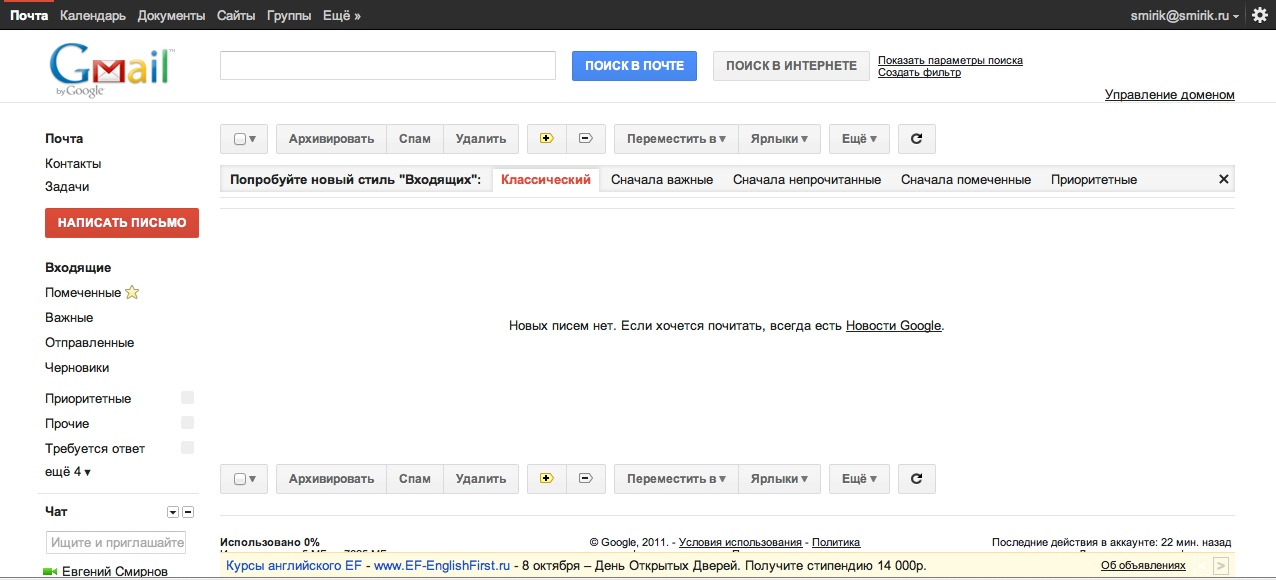
\includegraphics[width=1.0\textwidth]{images/gmail-new.jpg}}
\end{frame}

\subsection{Сервисы}
\begin{frame}
  \frametitle{G+}
	\centerline{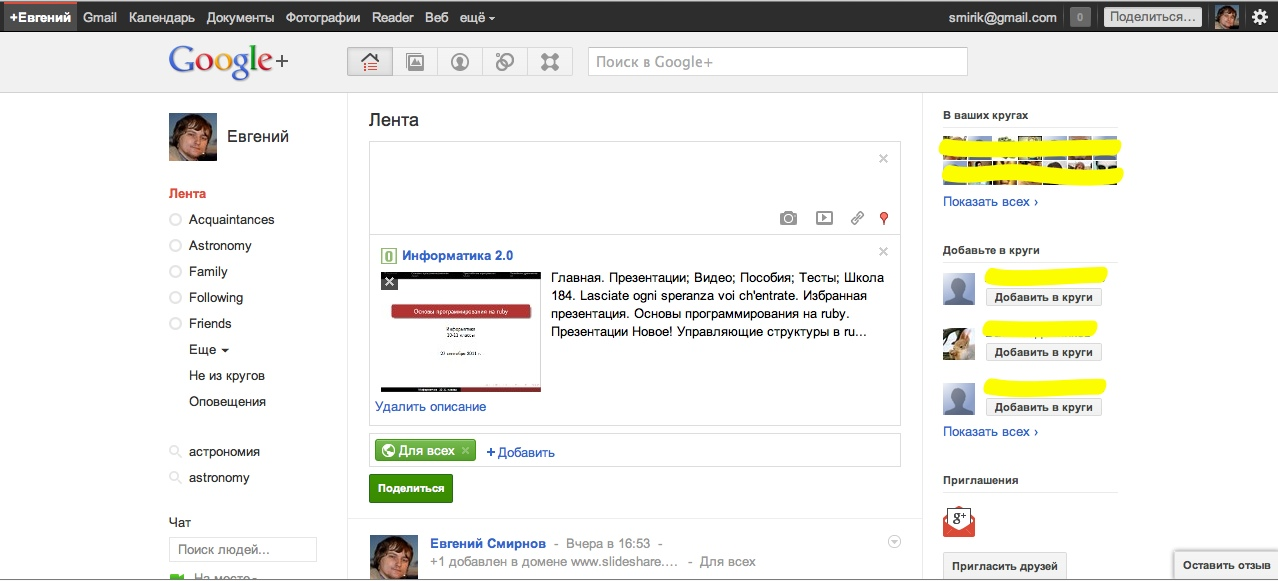
\includegraphics[width=1.0\textwidth]{images/gplus1.jpg}}
\end{frame}

\section{Google Docs}
\subsection{Сервисы}
\begin{frame}
  \frametitle{Google Docs}
	\centerline{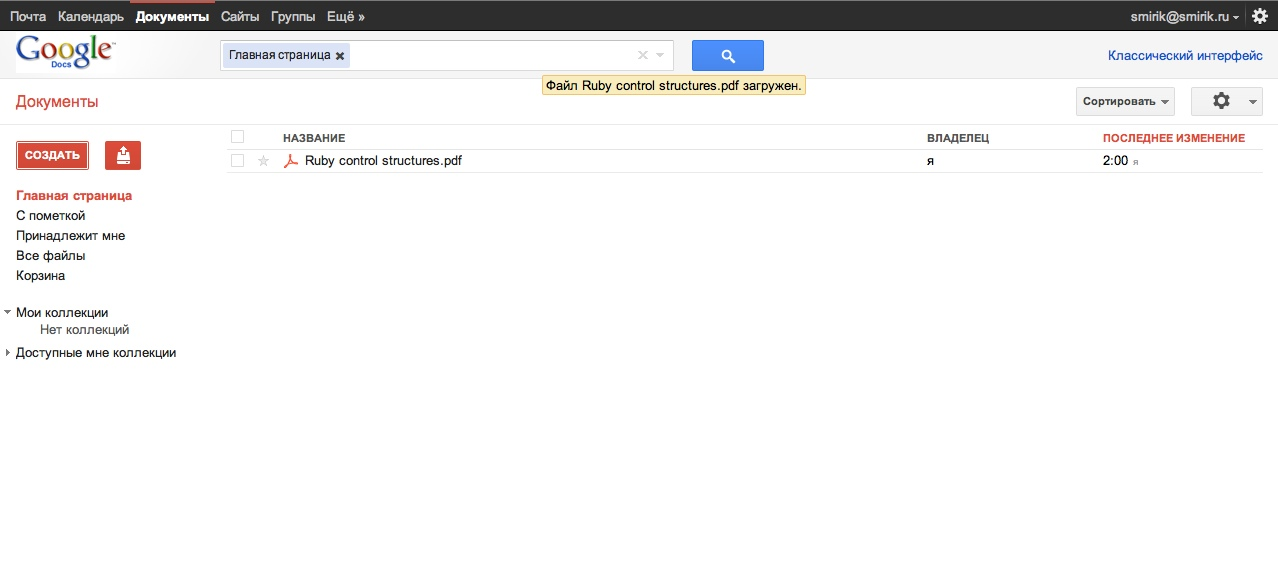
\includegraphics[width=1.0\textwidth]{images/gdocs1.jpg}}
\end{frame}

\subsection{Сервисы}
\begin{frame}
  \frametitle{Google Docs}
	\centerline{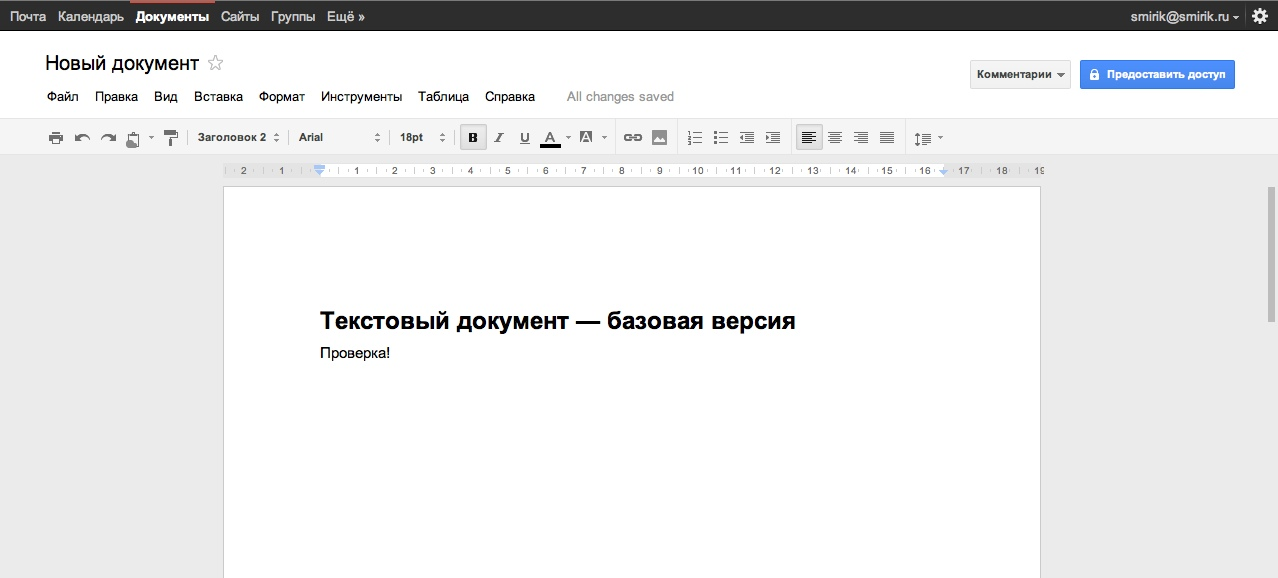
\includegraphics[width=1.0\textwidth]{images/gdocs2.jpg}}
\end{frame}

\subsection{Сервисы}
\begin{frame}
  \frametitle{Google Docs}
	\centerline{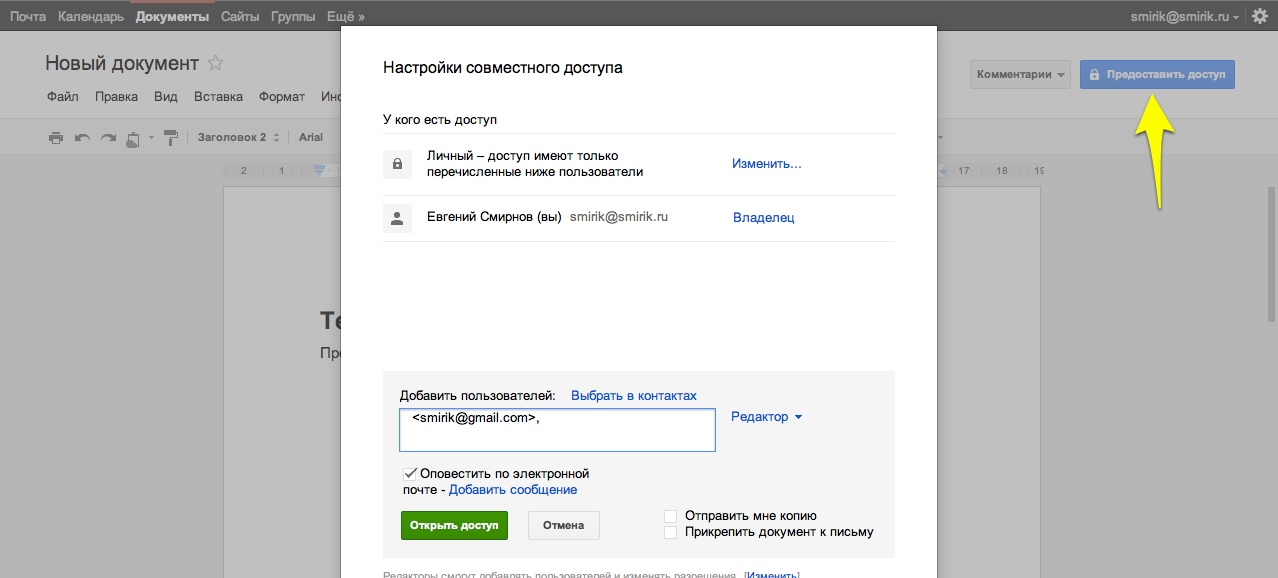
\includegraphics[width=1.0\textwidth]{images/gdocs3.jpg}}
\end{frame}

\subsection{Сервисы}
\begin{frame}
  \frametitle{Google Docs}
	\centerline{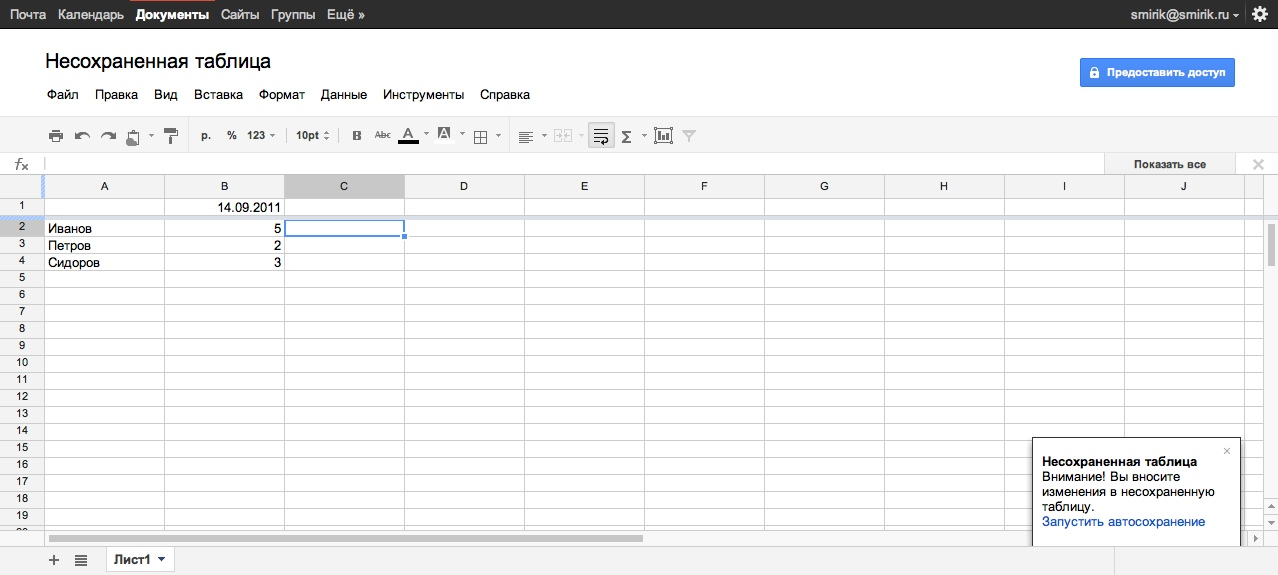
\includegraphics[width=1.0\textwidth]{images/gdocs4.jpg}}
\end{frame}

\subsection{Сервисы}
\begin{frame}
  \frametitle{Google Docs}
	\centerline{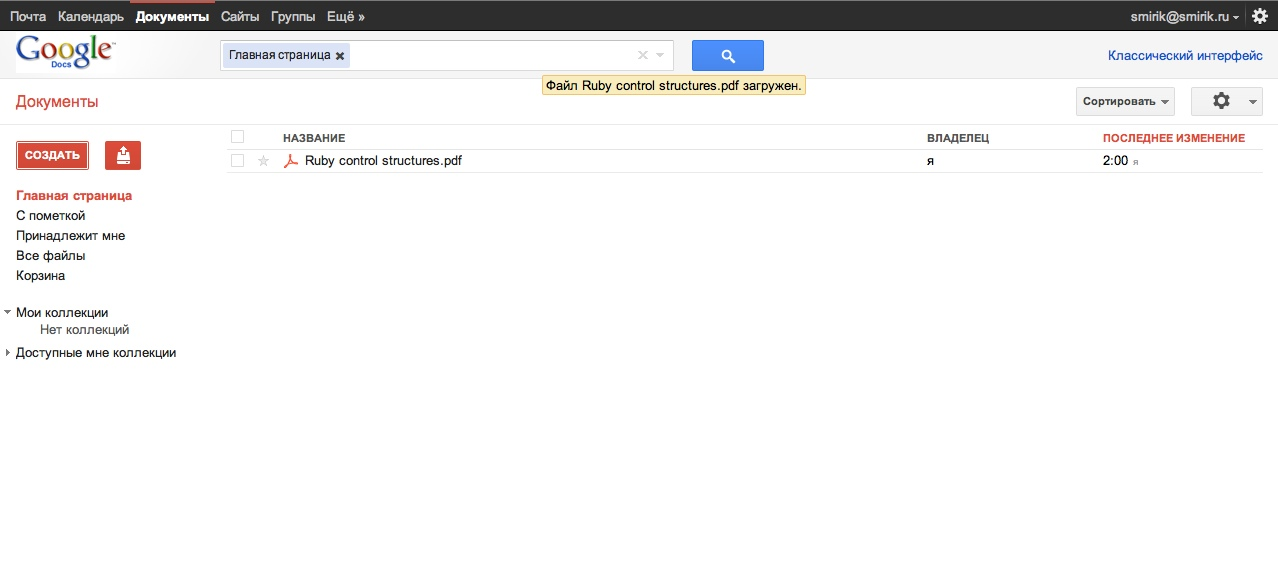
\includegraphics[width=1.0\textwidth]{images/gdocs1.jpg}}
\end{frame}

\section{Calendar + Reader}
\subsection{Сервисы}
\begin{frame}
  \frametitle{Google Calendar}
	\centerline{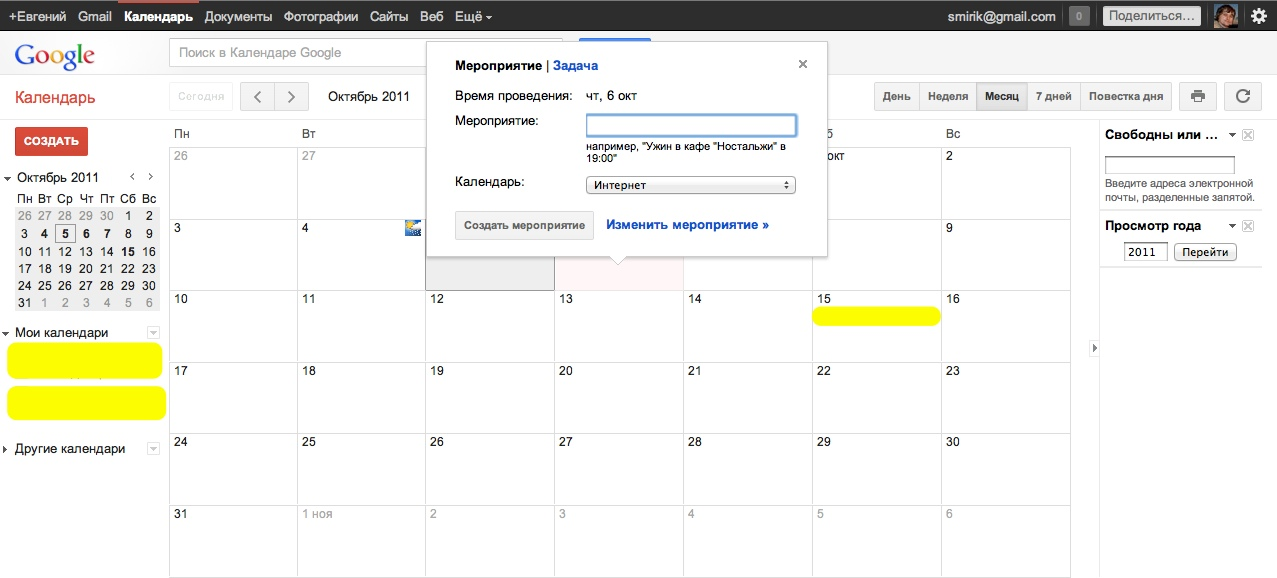
\includegraphics[width=1.0\textwidth]{images/calendar.jpg}}
\end{frame}

\subsection{Сервисы}
\begin{frame}
  \frametitle{Google Reader}
	\centerline{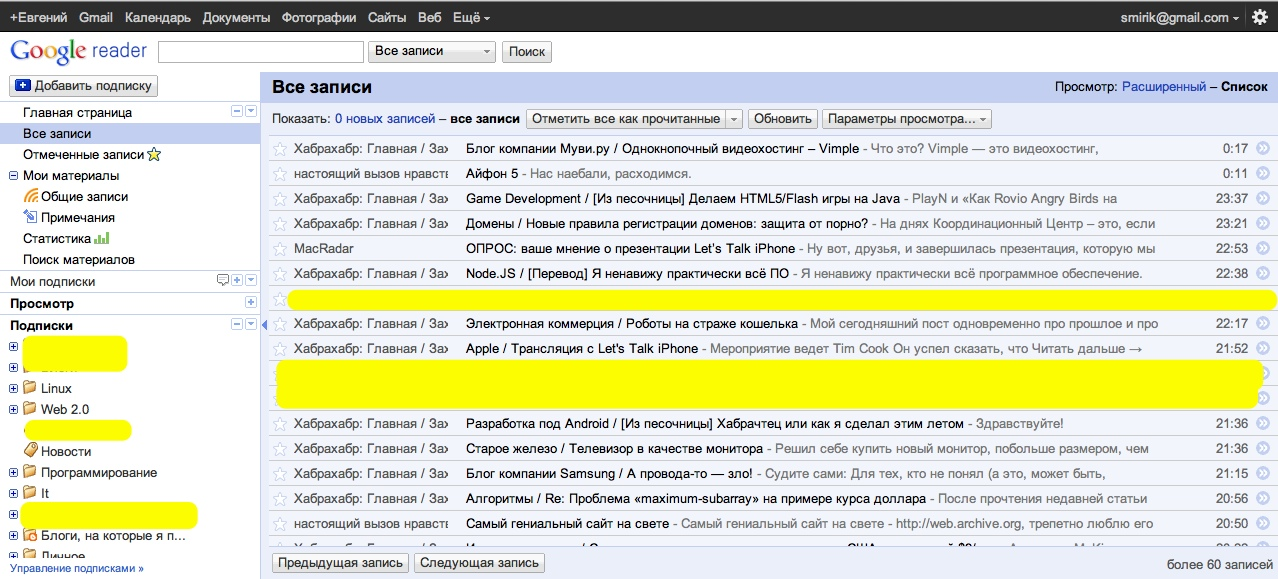
\includegraphics[width=1.0\textwidth]{images/reader.jpg}}
\end{frame}

\section{Blogger}
\subsection{Сервисы}
\begin{frame}
  \frametitle{Blogger}
	\centerline{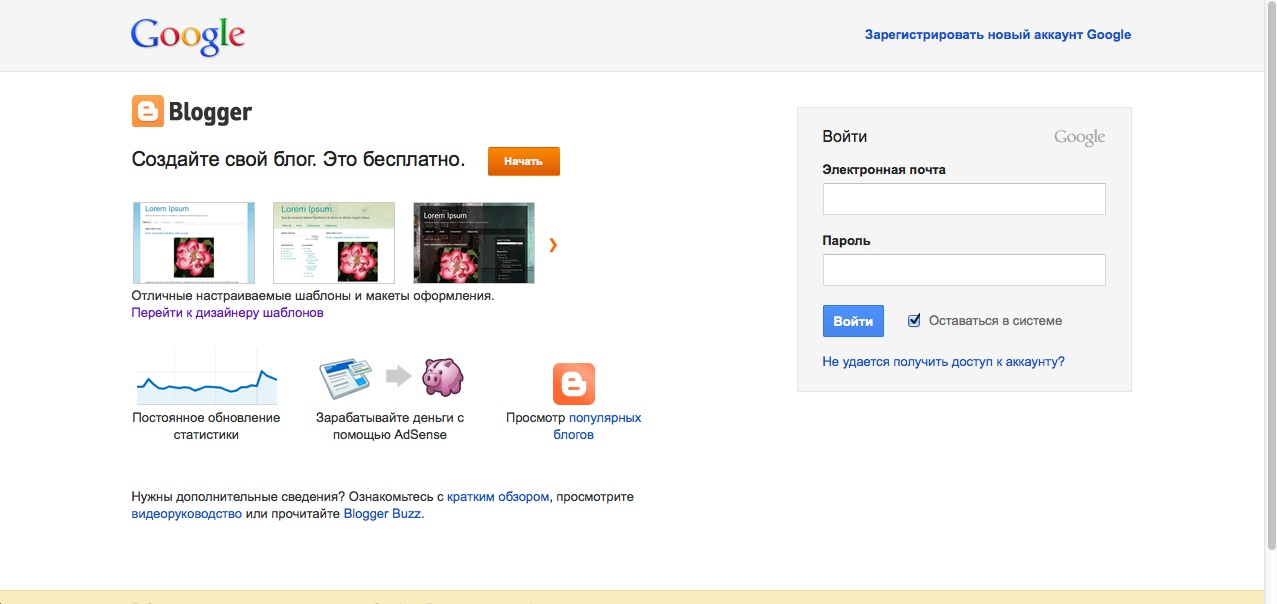
\includegraphics[width=1.0\textwidth]{images/blogger1.jpg}}
\end{frame}

\subsection{Сервисы}
\begin{frame}
  \frametitle{Blogger}
	\centerline{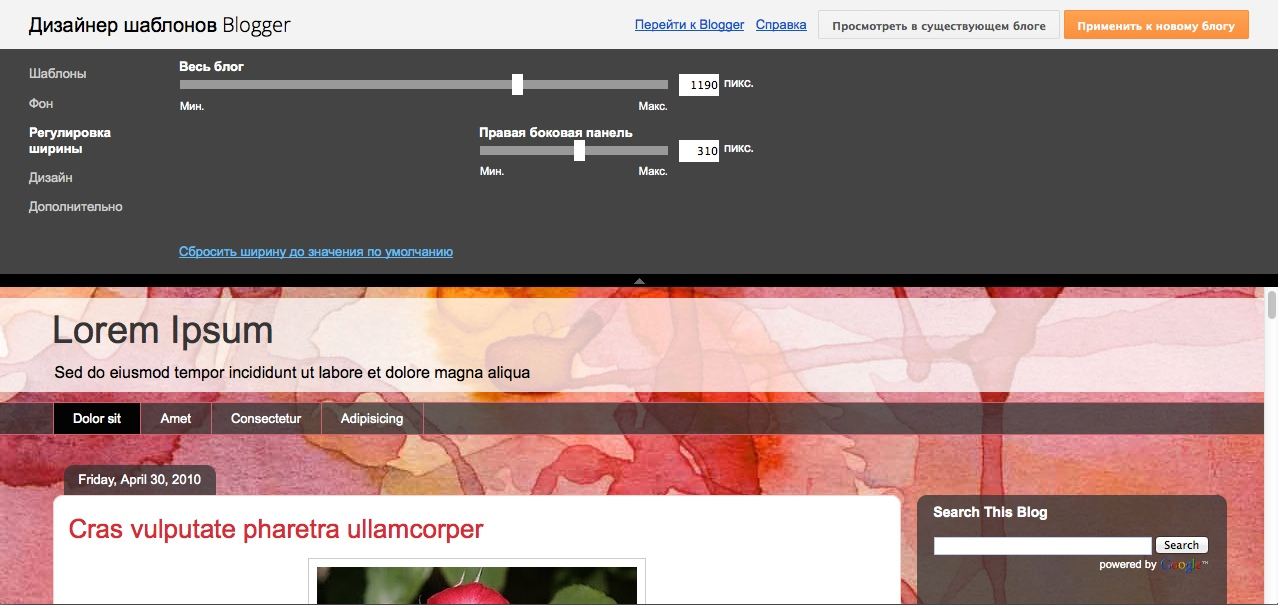
\includegraphics[width=1.0\textwidth]{images/blogger2.jpg}}
\end{frame}

\subsection{Сервисы}
\begin{frame}
  \frametitle{Blogger}
	\centerline{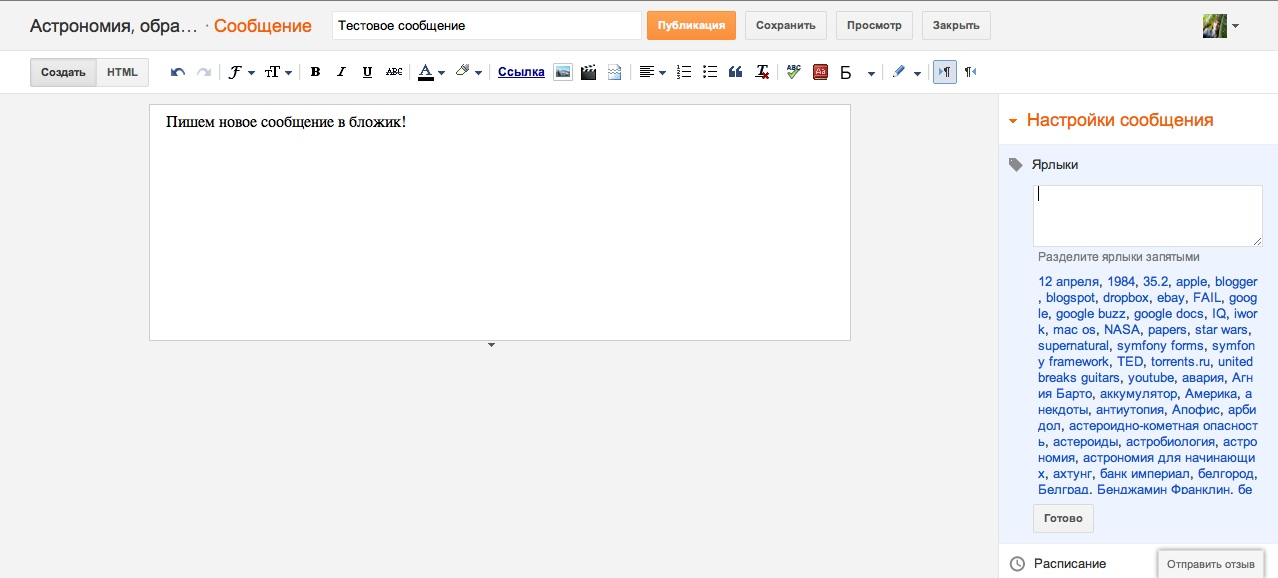
\includegraphics[width=1.0\textwidth]{images/blogger3.jpg}}
\end{frame}

\subsection{Сервисы}
\begin{frame}
  \frametitle{Blogger}
	\centerline{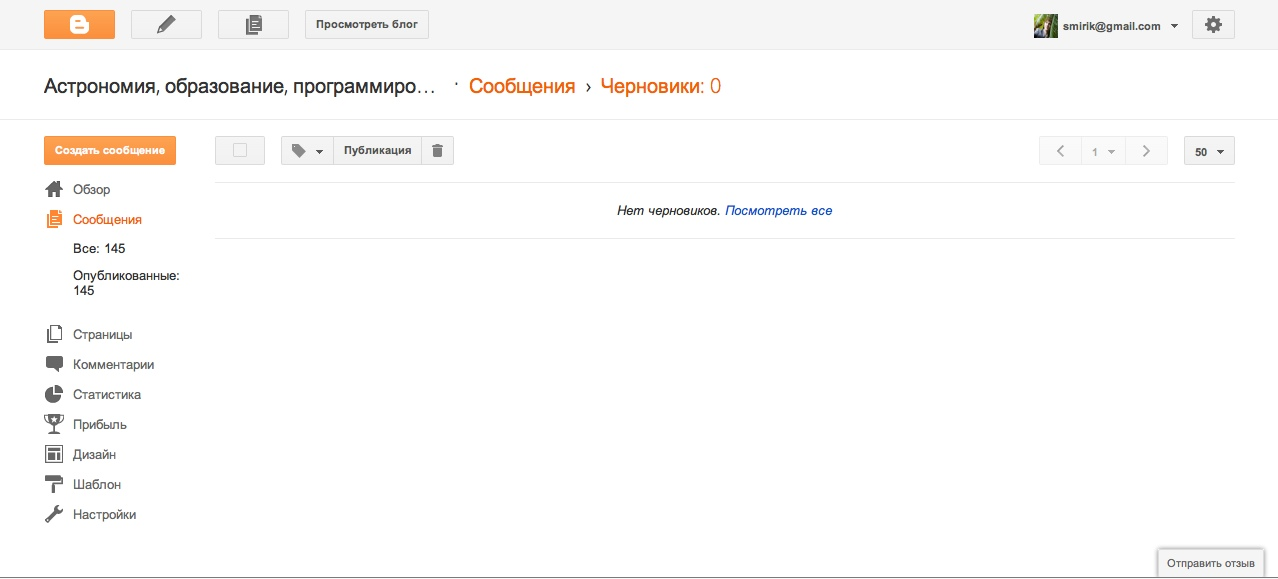
\includegraphics[width=1.0\textwidth]{images/blogger4.jpg}}
\end{frame}

\end{document}